\chapter{Materials \& Methods}
\label{chap:materials}

\begin{flushright}
 \textit{\textquotedblleft If you are afraid of change,
leave it here.\textquotedblright}\\
\textit{-- Seen on a tip box, Mountainview, CA}
\end{flushright}

\ifpdf
    \graphicspath{{6-MaterialMethods/Chapter6Figs/PDF/}}
\else
  \graphicspath{{6-MaterialMethods/Chapter6Figs/}}
\fi

\section{OpenFlow \& NOX}

OpenFlow is an open standard which enables a network engineer to control the behavior of their networking equipment programmatically. It represents a radical shift for the networking status quo. First,
manufacturers need to embrace OpenFlow and implement it\footnote{So far, HP,
NEC and Broadcom are known to have hardware implementations.}. Second, it
signals the end of distributed network algorithms and a return to simpler
centralized algorithms. 

OpenFlow and NOX are the basis for the implementation of the work in this Thesis. While the author believes that the future of computer networks lie alongside OpenFlow, he has implemented his work in a distributed manner in order to resemble current day network protocols.

\subsection{OpenFlow}
\label{sect:OPFW}

OpenFlow \cite{OPFW} offers a way for network researchers to try their
experimental protocols on real hardware and on the networks they use every day.
Until now there has been an extremely high barrier to entry for new networking
ideas due to the face that there is a rational reluctance within the community
to experiment with production traffic. The installed base of networking hardware has been largely built to conform with the extant RFC's and as such offers few, or no external interfaces. The result of this has been to exclude innovation since there is no mechanism to deploy or test alternative strategies to the ones laid down in silicon. Up until quite recently the only way that experimental progress could be made was work with specific experimental installation such as GENI \cite{GENI}. GENI is an nation-wide
(in the United States) network which provides programmable network elements via
virtualization and is capable of processing packets for multiple isolated
experiments. The disadvantage with such installations is that they are very
costly and take years to implement. Another example of such systems, while
smaller, are Emulab \cite{Emulab} and StarBed \cite{StarBed}.

There also exists several software solutions. Many OSs can route packets between
their interfaces and software implementation of routing protocols exist, for
example from XORP \cite{XORP} (eXtensible Open source Routing Platform).
Moreover, the CLICK \cite{CLICK} router project allows researchers to control
and manage the packet processing. While these solutions are interesting, they
do not provide the performance  or the port density required to test news ideas
efficiently. Hardware implementations are also available, the largest one is the
Advanced Telecommunications Computing Architecture Supercharged PlanetLab
platform \cite{PlanetLab} but it is targeted for large deployments and it is
extremely costly. There is also a NetFPGA \cite{NETFPGA} solution, but this
only provides four ports per card.

The question is why can we not find a way to use the hardware we
currently have and the networks we have deployed. This is exactly what OpenFlow
is designed to do.


\ifigure{Ofsign}{0.7}{The OpenFlow flow signature.}{fig:flowsign}

OpenFlow exploits the flow-tables contained in modern switches. Flow-tables are
built from TCAMs\footnote{A TCAM is a Ternary Content Addressable Memory. This
allows the operating system to match a third state, "X." The X state is a
"mask," meaning its value can be anything. This lends itself well to networking,
since netmasks operate this way. Routers can store their entire routing table in
these TCAMs, allowing for very quick lookups.}, which allow functions like QoS,
NAT, firewalls to run at line rate. OpenFlow stores the signature of a flow,
shown in Figure \ref{fig:flowsign} into the flow-table, and associates one or
more actions to be applied to the flow. The signature then allows the switch
to match subsequent packets onto that flow. The overall effect of the actions 
determines the behavior of the network. Figure \ref{fig:openflow} shows an
OpenFlow-enabled switch which is made up of a secure channel and a flow-table.
The secure channel connects the controller to the switch enables the controller
to send commands to the switch and manipulate its flow-table.

\ifigure{openflow}{0.5}{The OpenFlow switch.}{fig:openflow}

OpenFlow then provides an open and programmable interface to control the
contents of the flow-table. The set of actions which can be applied depend on whether
the switch implements all the actions or only the required ones. Moreover,
some manufacturers may not be able to implement certain actions due to their
underlying hardware as we will see in Section \ref{sect:NetHard}. The set of 
actions supported by an Openflow switch are summarized below:

\begin{itemize}
\item \textbf{Set VLAN ID} - Specify or overwrite the VLAN identifier.
\item \textbf{Set VLAN priority} - Define the priority of the packet with the VLAN.
\item \textbf{Strip VLAN header} - Remove all VLAN information.
\item \textbf{Modify source or destination MAC address} - Overwrite the Ethernet header information. 
\item \textbf{Modify source or destination IP address} - Overwrite the IP header information.
\item \textbf{Modify ToS bits} - Modify the Type of Service bits.
\item \textbf{Modify Transport source or destination ports} - Overwrite the TCP header information.
\end{itemize}

OpenFlow decouples the control from the datapath and exports it to a
controller, such as NOX, which will control the contents of the flow table. As an OpenFlow device is usually referred to as a switch even though technically it is not a stereotypical switch. OpenFlow can implement the function of a switch, router or even both; but it may also implement any other function. The term switch here is used to refer to the hardware on which OpenFlow is deployed.

\subsection{NOX}

NOX \cite{NOX} is an OpenFlow controller whose goal is to provide a programmatic
interface so that other applications can manage the underlying network. NOX
presents applications with a centralized programming model. NOX, programs are
written as if the network were contained on a single machine. NOX abstracts
low-level network details away from the developer. It essentially provides a
framework to manage OpenFlow-enabled switches and routers by handling the
low-level OpenFlow API provided by the enabled hardware.
 
A NOX based network is made up of openflow-enabled switches and one or more
instances of NOX where each instance provides the exact same network view to
the developer(s). Network applications are written on top of NOX and control
the behavior of the network by manipulating the flow-table. During normal
operation, NOX receives flow initiations (first packet of an unmatched flow),
these are passed by NOX to the network application which decides what to do
with such a flow. In the end, a new flow rule may be added to the flow table
and therefore subsequent matching flow will not be sent to NOX but rather the switch will apply the action specified in the added flow rule.

NOX's programmaable interface is driven by events, the namespace and the network
view. Traffic patterns in modern networks are constantly shifting therefore
flows come and go, links go up and down. NOX handles this by allowing developers
to register for events. When an event occurs NOX calls the handler passed at
the registration. 
  
NOX builds a network view based on messages obtained from the Openflow-enabled
switches as they connect. Applications use the network view to perform
computations or decide how to handle a certain type of packet, etc. Each NOX
instance constructs a list of loaded applications and from this point onwards
each loaded application can exchange messages with each other. This is known
as the NOX namespace. 
	

\section{TestBed Installation}

\subsection{Routing Hardware}
\label{sect:NetHard}

The testbed is implemented on HP Procurve switches [procurve] running an
experimental OpenFlow-enabled firmware. OpenFlow on the HP platform is
instantiated per VLAN\footnote{Virtual Local Area Network}. We have exploited
this by defining different VLANs on each network device which are then used to
identify the network address range controlled by the device. The VLAN ID is
then advertised to the controller who uses it to assign a virtual gateway
address for each router in the network. 

The HP implementation of OpenFlow has several limitations which are mostly due
to the underlying hardware. For example, HPs cannot perform mac address
rewriting in hardware because their routing support is monolithic and the
re-writing functionality cannot be isolated from the other routing
functionality. It is actually more limiting, HPs can only re-write mac-addresses
to a single mac address (the base address of the device) and therefore
specifying a custom mac address is impossible. Since the hardware does not
support some OpenFlow actions, they are implemented by the OpenFlow firmware in
software. As the processor within switches is a shared resource between all the
ports and is not very powerful in the first place, the software path is a
very slow path. Our measurements show that the software path provides roughly
1.25 MB/s overall bandwidth per switch, this is equivalent to 10Mb/s cross
sectional bandwidth. 

Since we are designing a new routing protocol which is supposed to surpass all
existing ones in terms of performance, using our OpenFlow devices in software
path (ie. invoking the switch CPU) is counter productive. Therefore we have employed several workarounds in
order to build a routing protocol using HP's OpenFlow implementation.

\begin{figure}
  \centering
  \subfloat[Standard routing model.]{\label{fig:normalrouting}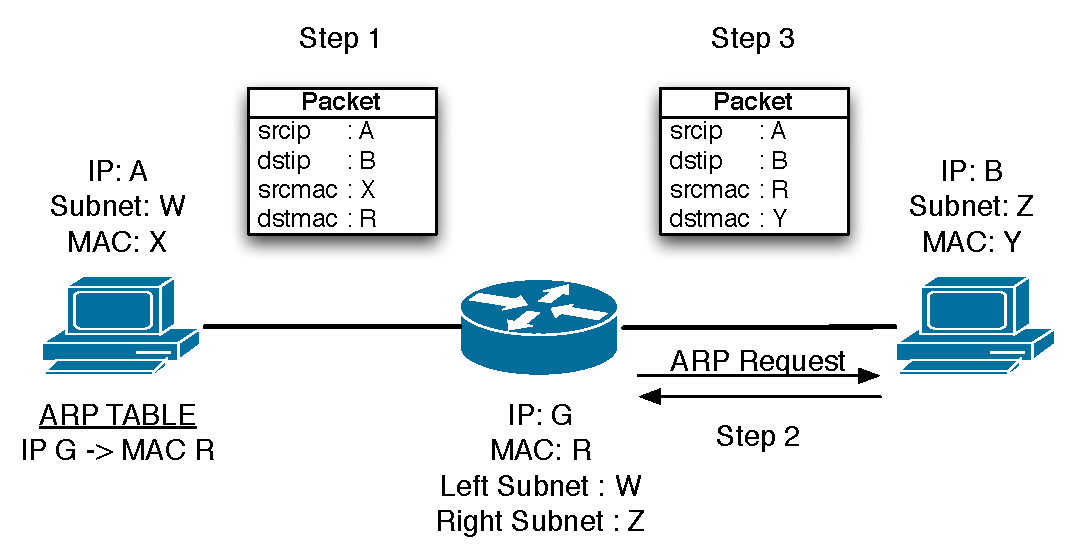
\includegraphics[width=\textwidth]{normalrouting}}
  \\                
  \subfloat[HP Openflow Routing.]{\label{fig:HProuting}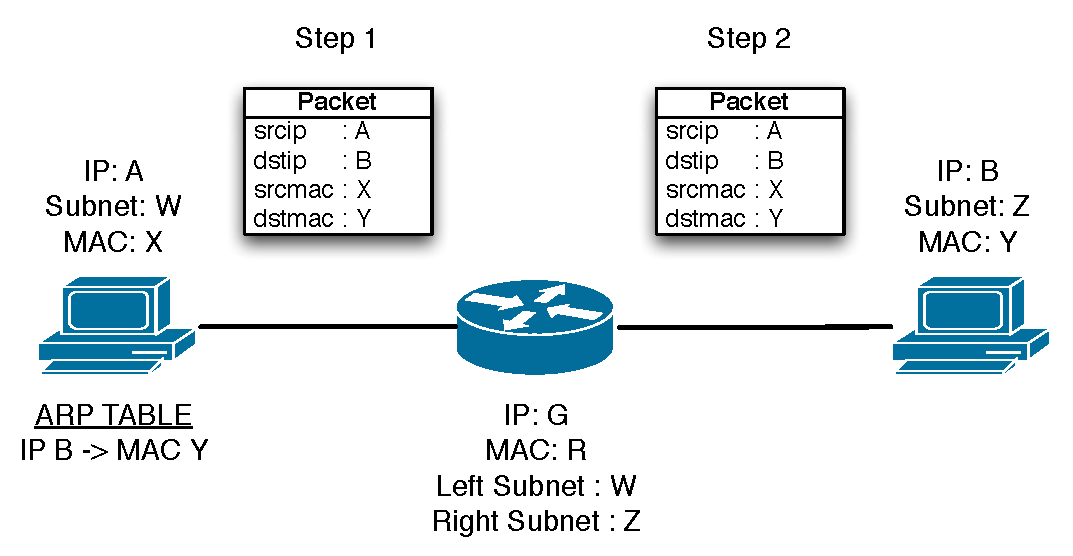
\includegraphics[width=\textwidth]{HProuting}}
  \caption{An explanation of routing processes.}
  \label{fig:routing}
\end{figure}

Our goal is to develop a protocol which achieves its routing function without
replacing the Link Layer information, which is mainly how a router behaves
\cite{RFC1812}. The Link Layer information is replaced by a router in order to
be able to direct a packet to its next-hop whilst maintaining the source and
destination IP fields intact. This is easily solved in an OpenFlow
implementation as we can direct packets out of any interface at any moment. The
more crucial problem arises when the packet is arriving at its destination.
Because we will not be able to re-write the MAC address, which is set to the
MAC address of the last-hop router, the destination host will reject the
packet. The workaround here is rather cumbersome, we prepopulate each host ARP
table with the IP to MAC address mappings, and therefore when a host sends
out a packet to any other host it can already set the destination MAC address
to its final value. These two workarounds allow us to design a routing
protocol albeit slightly simplified but the main routing function, of routing
packets through a network via the most efficient path, is still guaranteed.
Figure \ref{fig:normalrouting} depicts the normal behavior of a router and Figure
\ref{fig:HProuting} shown the behavior of routing in our OpenFlow testbed. In
Figure \ref{fig:normalrouting}, a host with IP address A sending traffic to
another host with IP B would first notice that due to its subnet mask that the
destination IP is not on the same local area network (LAN). Therefore, it builds
a packet with source and destination IP A and B respectively and source and
destination MAC address X and R respectively (Step 1).  When the packet arrives
at the router, the router performs an ARP request to determine the MAC address
associated to IP B (Step 2). Once the MAC address is resolved, the router
rewrites in the packet and sends the packet to the destination (Step 3). In
Figure \ref{fig:HProuting}, since the HP Openflow firmware is not able to do any
re-writing (efficiently, at least), we prepopulate the ARP table at every host
for all other hosts. This results in that the packet built at Step 1 already
contains the correct MAC address for the destination IP. Therefore, the router
performs no MAC address lookup and simply forwards the packets to the
destination (Step 2).

%%%SUBFIG ROUTING!!!

\subsection{Network Installation}

\ifigure{TestBed}{0.6}{The testbed as it is implemented at CERN's computing center.}{fig:testbedreal}

The testbed, shown in Figure \ref{fig:testbedreal}, is designed to provide isolated connectivity for OpenFlow experiments while providing hosts and network testers (see
Section \ref{sect:GETB} for experimental evaluation). This is achieved by
deploying connectivity via three networks. First, comes the connection to CERN's
General Purpose Network (GPN), then there is the Control Network (CN) and
finally the OpenFlow network (OF). 

%\begin{figure}
  %\centering
  %\subfloat[The testbed as it is implemented at CERN's computing center.]{\label{fig:testbed}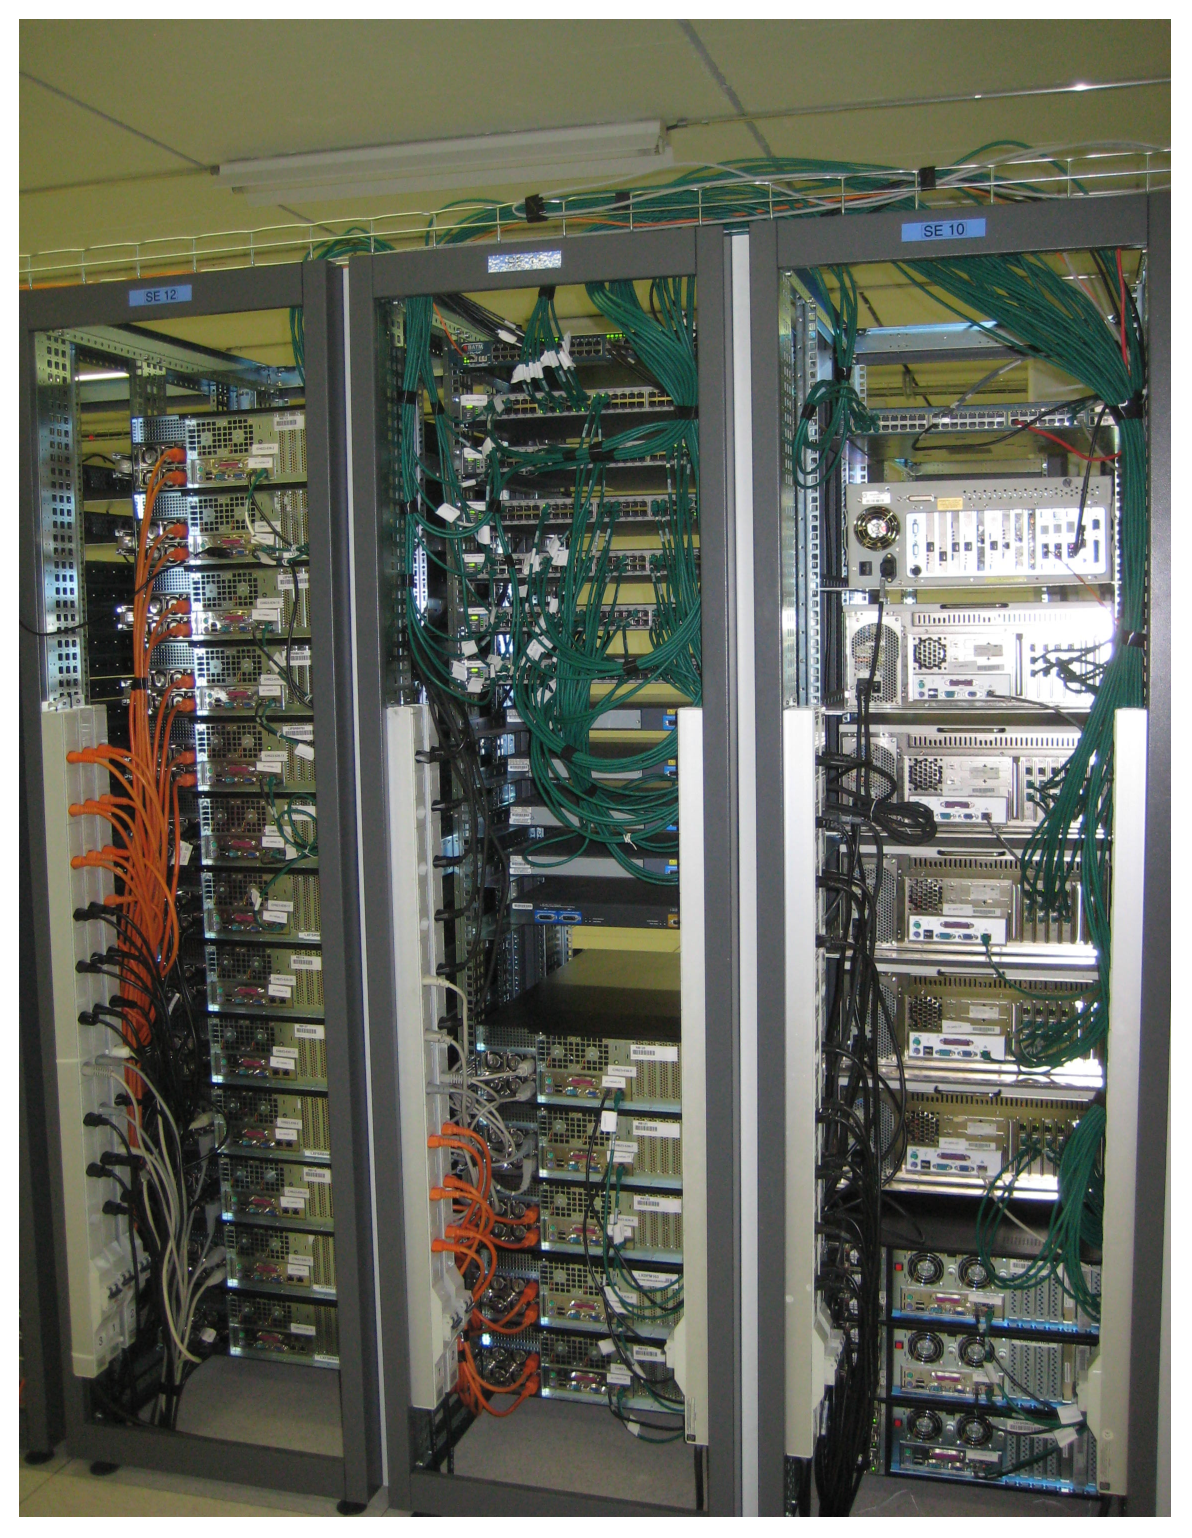
\includegraphics[width=0.5\textwidth]{testbed}}   \\             
 % \subfloat[The connectivity map of the Testbed.]{\label{fig:schema}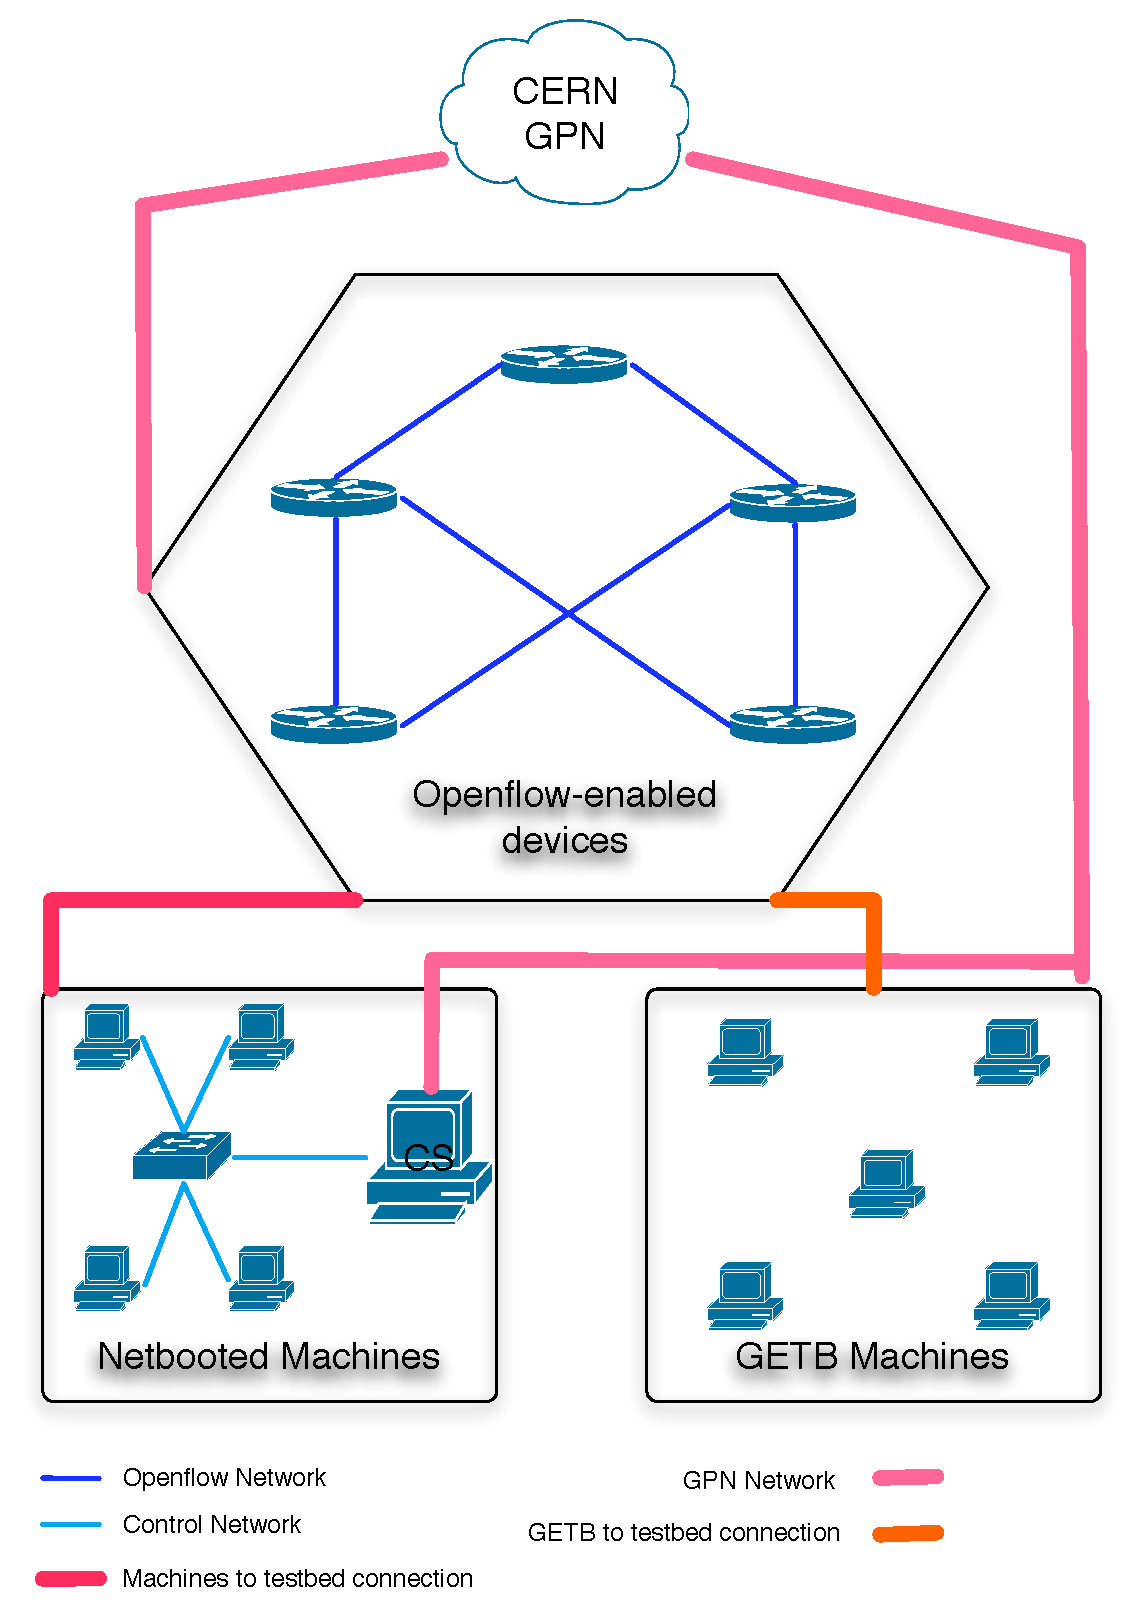
\includegraphics[width=0.7\textwidth]{TestbedSchema}}
 % \caption{The testbed in CERN.}

%\end{figure}



Figure \ref{fig:schema} shows the block connectivity map used with our testbed. The GPN provides connectivity to the world which allows us to install software
on the hosts and update the firmware running on the switch devices. The CN is
the command and control network, which provides the Network FileSystem
(NFS) where the data and systems are stored for the hosts. The GETB Machines (see \ref{sect:GETB} for a complete description) are installed as individual machines each connected to the GPN via its own interface. The OF is the actual connectivity which defines the topology of our test network, as shown in Figure \ref{fig:schema}.

\ifigure{TestbedSchema}{0.5}{The connectivity map of the Testbed.}{fig:schema}

\subsection{Machine deployment}

The hosts are netbooted\footnote{Netbooting consists in booting machines from a
server over the network. These machines can either be diskless or not, but all
the boot information is contained on the network server.} from the Central
Server (CS). Each is configured to obtain an IP address at boot time via the
Dynamic Host Configuration Protocol (DHCP). DHCP provides the hosts
with extra information such as the gateway address, and the netbooting
server. The host downloads a bootloader from the netbooting server and boots as
if it had the bootloader locally. The bootloader instructs the host to mount an
NFS volume where all the boot and data for the host to run is contained. For
more information on netbooting, the reader is referred to \cite{Netboot}.

Each host has a dedicated directory on the CS which contains the specific
configuration of that particular host. Therefore, each host behaves as a
diskless machine and pulls its root filesystem from the CS. This approach has
several advantages. First, the configuration of the hosts is simplified as
they can all be done on the CS. Second, deployment of a new machine is accelerated as
we can simply copy another hosts' directory and modify the configuration. Third,
since the directory containing all the applications used by the hosts is shared
by all the hosts, we just need to install application into this directory and
it is directly available on all the hosts.

\section{GETB Network Testers}
\label{sect:GETB}

The Gigabit Ethernet TestBed \cite{GETB} (GETB) is a FPGA-based platform
designed to provide a flexible and fully programmable device testing environment.
The GETBs were designed to deliver full 1Gb/s wire speed full duplex for two ports running concurrently.

Modifications to the FPGA firmware are difficult and time consuming. This is why
the GETB was programmed to offer services. A set of relatively simple
functions were implemented in the FPGA. These were then used as building blocks
for more complex behavior – the hardware functions were accessible to the user
through the GETB control software (GETB/CS).
   
The aim of the GETB/CS was to provide a common control infrastructure for all
the GETB-derived projects. We needed a system flexible enough to allow complete
customization for the different applications. We also wanted to be able to
easily automate the actions of the GETB cards. This requirement practically
excluded the development of a Graphical User Interface specifically for the
GETB (which we thought would limit the functionality and would be difficult
to maintain and further improve). Finally, our decision was to build almost all
the GETB control system using the Python scripting language \cite{Python}.

The GETB/CS is divided into two main components: the server component – which
runs on the computers hosting GETB cards; and the client component running on
any other machine which needs to access the resources of the servers. Each
machine which contains GETB cards runs the server component. Then, the client
is run on a different machine and controls the operation of the GETB cards.

The GETB cards enable you to generate traffic at various rates and in a
controlled fashion. Therefore, we are able to devise test scenarios with a relatively
large port density as we can connect up to 32 GETB simultaneously.


\section{Experimental Technique}

Now that we have described our experimental testbed setup and and the
associated network tester, we are going to briefly define the methods used to
test our protocols. 

\subsection{Parasite Traffic}

In this test, we measure the capacity of the network device to forward traffic
in the presence of interfering traffic. This test will indicate the capacity of
the router to avoid areas with pre-existing congestion.

\subsection{Fully Meshed Traffic}

Fully meshed traffic, in which traffic is transmitted from all active
ports to all other active ports. This will allow us to determine the
drop-rates and throughput.

\subsection{Latency}

In this scenario the idea is to measure the time required to transmit a packet
from one host to another while the network is transporting traffic at different
rates. Doing so will bring out the capability of the routing protocol to route
traffic efficiently and through the current best path.

\section{Summary}

In this section, we have presented the tools which have enabled us to develop our congestion-aware protocols. Moreover, we have introduced the technologies which allow us to deploy our testbed and end nodes. Finally, we have described our tester boards which will generate the traffic we need to test our protocols. The next section will present the results obtained from our test environment.
